\documentclass[twoside,a4paper]{report}

\usepackage[bottom]{footmisc}
\usepackage[pdftex]{graphicx}
\usepackage{textcomp}
\usepackage[compact,nobottomtitles*]{titlesec}
\titleformat{\chapter}[display]
{\normalfont\bfseries}{}{0pt}{\huge}
\usepackage{lipsum}
\usepackage{wrapfig}
\usepackage{adjustbox}
\usepackage[utf8]{inputenc}
\usepackage[english,main=polish]{babel}
\usepackage[T1]{fontenc}
\usepackage[fit]{truncate}
\usepackage{array}
\usepackage{makecell}
\usepackage{float}
\usepackage{anysize}
\usepackage{enumitem}
\usepackage[font=small,labelfont=bf]{caption}
\usepackage{subcaption}
\usepackage{url}
\usepackage{hyperref}
\usepackage{csquotes}
\usepackage[
sorting=none
]{biblatex}
\emergencystretch=1em
\addbibresource{bibliografia.bib}
\usepackage{listings}
\renewcommand{\ttdefault}{pcr}
\usepackage{fancyhdr}
\usepackage{multirow}
\usepackage{tabularx}
\usepackage{ltablex}
\usepackage{indentfirst}
\usepackage{gensymb}
\raggedbottom

\newcolumntype{C}{>{\centering\arraybackslash}X}

\newcommand*{\noaddvspace}{\renewcommand*{\addvspace}[1]{}}
\addtocontents{lof}{\protect\noaddvspace}

\pagestyle{fancy}
\fancyhf{}

\renewcommand{\lstlistlistingname}{Spis listingów}

\lstdefinelanguage{JavaScript}{
    keywords={function, class, extends, return, render},
}

\lstdefinelanguage{Elm}{
    keywords={type, alias, update, case, of, init, view, subscriptions, let, in, viewDate, viewTime},
}

\lstset{
  basicstyle=\ttfamily,
  keywordstyle=\textbf,
  columns=fullflexible,
  frame=single,
  breaklines=true,
}

\renewcommand{\chaptermark}[1]{\markboth{#1}{}}
\renewcommand{\sectionmark}[1]{\markright{\thesection\ #1}}
\renewcommand{\headrulewidth}{0.5pt}
\renewcommand{\footrulewidth}{0pt}

\fancyhead[LE,RO]{\bfseries\thepage}
\fancyhead[LO]{\nouppercase{\bfseries{\truncate{.95\headwidth}{\rightmark}}}}
\fancyhead[RE]{\nouppercase{\bfseries{\truncate{.95\headwidth}{\leftmark}}}}

\titlespacing*{\chapter}{0pt}{-50pt}{20pt}

\linespread{1.5}

\parskip0.05in

\marginsize{3.5cm}{2.5cm}{2.5cm}{2.5cm}
\fancyhfoffset[E,O]{0pt}

% ---------------------------------------------------------------------------------------------------------------------

\begin{document}

\chapter{Instrukcja laboratoryjna}
W poniższym rozdziale przedstawiam przykładową instrukcję laboratoryjną, która krok po kroku przeprowadza czytelnika przez proces tworzenia aplikacji w Elmie, zaczynając od przygotowania środowiska deweloperskiego, przez podstawy języka wraz z ćwiczeniami pozwalającymi na lepsze zrozumienie składni, aż po stworzenie większej aplikacji frontendowej.

\section{Przygotowanie środowiska}
Pierwszą rzeczą, którą należy się zająć przed rozpoczęciem nowego projektu jest przygotowanie odpowiedniego środowiska deweloperskiego.
Należy upewnić się, że wszystkie narzędzia potrzebne do wykonania pracy są zainstalowane i prawidłowo skonfigurowane.
W przypadku pracy z Elm'em zalecane będzie korzystanie przede wszystkim z platformy dostarczanej przez autora, edytora tekstu wspierającego podświetlanie składni, a także innych narzędzi wspomagających proces tworzenia oprogramowania z użyciem tej technologii.

\subsection{Platforma Elm}
Najważniejszą rzeczą, jaka będzie potrzebna podczas pracy z Elm'em, będzie platforma języka zawierająca m.in.~takie narzędzia jak kompilator oraz menadżer bibliotek.
Poniżej przedstawiam instrukcję instalacji tej platformy na systemach operacyjnych Linux i Windows.
Po przejściu tych kroków, w wierszu poleceń należy wykonać instrukcję \texttt{elm}.
Jeśli wszystko zostało prawidłowo zainstalowane i skonfigurowane, na ekranie powinien pojawić się widok podobny do przedstawionego na rysunku~\ref{fig:elm_output}.

\begin{figure}[H]
    \centering
    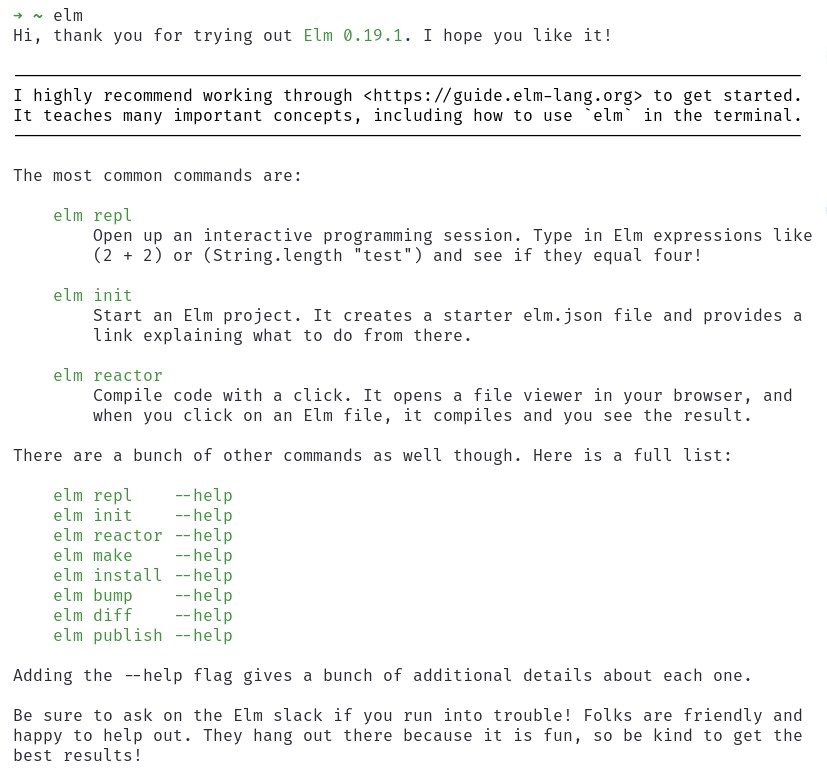
\includegraphics[width=0.95\textwidth]{img/elm_output.png}
    \caption{Wyjście instrukcji \texttt{elm}}\label{fig:elm_output}
\end{figure}

\subsubsection{Linux}
Najprostszym sposobem instalacji platformy Elm na systemie operacyjnym Linux jest wykorzystanie narzędzia \texttt{npm}~-- powszechnie używanego menadżera pakietów służącego do zarządzania warstwą frontendową aplikacji internetowych.
Aby zainstalować \texttt{npm} należy skorzystać z systemowego menadżera pakietów.
Na przykładzie dystrybucji Ubuntu będą to komendy:

\begin{lstlisting}
  $ sudo apt update
  $ sudo apt install npm
\end{lstlisting}

Kiedy narzędzie zostanie już pomyślnie zainstalowane, można przejść do instalacji platformy Elm.
Posłuży do tego polecenie:

\begin{lstlisting}
  $ npm install -g elm
\end{lstlisting}

Zgodnie z dokumentacją \texttt{npm}~\cite{npmdocs}, flaga \texttt{-g} oznacza, że pakiet zostanie zainstalowany globalnie, dzięki czemu będzie dostępny z każdego miejsca z systemu.
Aby sprawdzić, czy rzeczywiście tak się stało, wystarczy w wierszu poleceń uruchomić komendę \texttt{elm}.
Jeżeli wszystkie kroki przebiegły pomyślnie, na ekranie powinien ukazać się widok podobny do przedstawionego na rysunku~\ref{fig:elm_output}, tak jak zostało to już wcześniej wspomniane.

\subsubsection{Windows}
Osoby korzystające z systemu operacyjnego Windows mogą skorzystać z npm, tak jak to było opisane w powyższej sekcji dotyczącej Linuxa lub posłużyć się dedykowanym \href{https://github.com/elm/compiler/releases/download/0.19.1/installer-for-windows.exe}{instalatorem Elm'a}~\cite{elm_installer} na system Windows.
W tym drugim przypadku wystarczy przejść przez wszystkie kroki zostawiając opcje domyślne i w rezultacie Elm zostanie pomyślnie zainstalowany i będzie gotowy do użytkowania.
W celu sprawdzenia czy faktycznie tak się stało, należy uruchomić wiersz poleceń oraz wykonać instrukcję \texttt{elm}.
Wyjście komendy powinno być podobne do tego przedstawionego na rysunku~\ref{fig:elm_output}, tak jak zostało to już wcześniej wspomniane.

\subsection{Edytor}
Ważnym elementem tworzenia oprogramowania jest wyposażenie się w odpowiedni edytor tekstowy, który jest w stanie podświetlać składnię języka, z którego aktualnie korzystamy.
Żeby osiągnąć ten cel, w przypadku Elm'a potrzebna będzie instalacja dodatkowej wtyczki do jednego z następujących edytorów:

\begin{itemize}[noitemsep,topsep=0pt]
    \item{\href{https://atom.io/packages/language-elm}{Atom}}
    \item{\href{https://github.com/jcollard/elm-mode}{Emacs}}
    \item{\href{https://github.com/klazuka/intellij-elm}{IntelliJ}}
    \item{\href{https://github.com/rundis/elm-light}{Light Table}}
    \item{\href{https://github.com/evancz/elm-syntax-highlighting/}{Sublime Text}}
    \item{\href{https://github.com/elm-tooling/elm-vim}{Vim}}
    \item{\href{https://github.com/elm-tooling/elm-language-client-vscode}{VS Code}}
\end{itemize}

Powyższa lista zawiera odnośniki do wspomnianych wtyczek dla danego edytora, wystarczy kliknąć nazwę swojego ulubionego edytora i pobrać odpowiedni dodatek.
Na potrzeby niniejszej instrukcji przedstawię proces instalacji wtyczki dla edytora Visual Studio Code~\cite{vscode}, ponieważ jest to jedno z najbardziej powszechnie używanych narzędzi do pracy z kodem źródłowym.

W tym celu należy otworzyć edytor VS Code, otworzyć konsolę \textit{Quick Open} przy pomocy skrótu \textit{Ctrl+P} i wpisać następującą komendę:
\begin{lstlisting}
  ext install Elmtooling.elm-ls-vscode
\end{lstlisting}
Wtyczka powinna zostać automatycznie zainstalowana i dalsza konfiguracja nie jest konieczna, edytor powinien być gotowy do pracy.
Po instalacji można przejść do kolejnego kroku.

\subsection{Tworzenie projektu}
Elm jest dostarczany wraz z zestawem bardzo przydatnych narzędzi.
Jednym z nich jest \texttt{elm init}, które posłuży nam do stworzenia nowego projektu.
W tym celu należy otworzyć wiersz poleceń i wykonać następujące instrukcje:

\begin{lstlisting}
  $ mkdir lab
  $ cd lab
  $ elm init
\end{lstlisting}

Po wypisaniu zawartości katalogu \texttt{lab} z użyciem polecenia \texttt{ls} powinny pojawić się dwa nowe elementy:

\begin{itemize}[noitemsep,topsep=0pt]
    \item{Plik \texttt{elm.json} opisujący projekt oraz jego zależności}
    \item{Katalog \texttt{src/} zawierający nasze przyszłe pliki Elm'a}
\end{itemize}

Następnym krokiem będzie utworzenie nowego pliku \texttt{Main.elm} w nowo utworzonym katalogu \texttt{src/}.
Będzie się tam znajdował kod aplikacji, która zostanie stworzona w kolejnych krokach.

\section{Podstawy języka Elm}
W celu nauki podstaw języka Elm użyte zostanie narzędzie \texttt{elm repl}, pozwalającego na korzystanie z interaktywnej sesji programistycznej.
Należy otworzyć wiersz poleceń i wpisać polecenie \texttt{elm repl}.
Powinien ukazać się widok podobny do przedstawionego na rysunku~\ref{fig:elm_repl_output} poniżej.

\begin{figure}[H]
    \centering
    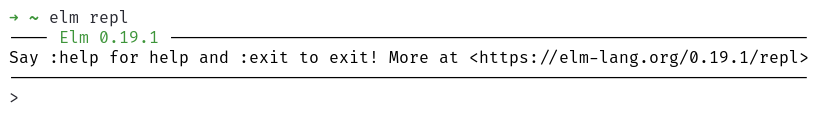
\includegraphics[width=0.95\textwidth]{img/elm_repl_output.png}
    \caption{Otwarta interaktywna sesja \texttt{elm repl}}\label{fig:elm_repl_output}
\end{figure}

\subsection{Wartości}
Najmniejszym budulcem aplikacji w Elmie są \textbf{wartości}.
Mogą to być liczby, ciągi znaków, czy typy logiczne, np. 10,~,,Hello'', True.
Po wpisaniu do okna \texttt{elm repl} danej wartości, na ekranie powinna zostać pokazana powtórzona wartość, a po dwukropku jej typ.

Wartości można także łączyć z operatorami.
Dla liczb będą to typowe operatory matematyczne, jak \texttt{+}, \texttt{-}, \texttt{*}, \texttt{/}, dla ciągów znaków operatorem konkatenacji jest \texttt{++}, a dla typów logicznych dostępne są operatory logiczne~,,\texttt{\&\&}'' (AND) oraz~,,\texttt{||}'' (OR).

Na rysunku~\ref{fig:repl_values} pokazane zostały przykłady efektów takich wywołań.

\begin{figure}[H]
    \centering
    \begin{subfigure}{.29\textwidth}
        \centering
        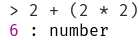
\includegraphics[height=1cm]{img/repl_number}
        \caption{Liczba}\label{fig:repl_number}
    \end{subfigure}
    \begin{subfigure}{.4\textwidth}
        \centering
        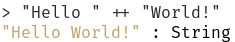
\includegraphics[height=1cm]{img/repl_string}
        \caption{Ciąg znaków}\label{fig:repl_string}
    \end{subfigure}
    \begin{subfigure}{.29\textwidth}
        \centering
        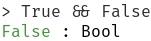
\includegraphics[height=1cm]{img/repl_bool}
        \caption{Typ logiczny}\label{fig:repl_bool}
    \end{subfigure}
    \caption{Wartości w Elmie}\label{fig:repl_values}
\end{figure}

\subsection{Funkcje}
\begin{wrapfigure}{r}{0.45\textwidth}
    \centering
    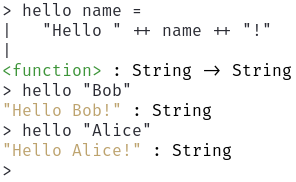
\includegraphics[width=0.45\textwidth]{img/repl_func}
    \caption{Definicja funkcji w Elmie}\label{fig:repl_func}
\end{wrapfigure}

Funkcje w Elmie określają, w jaki sposób wartości mogą zostać przetworzone.
Na rysunku~\ref{fig:repl_func} pokazana została przykładowa funkcja \texttt{hello}, która przyjmuje argument \texttt{name} i zwraca nowy ciąg znaków.

Można zauważyć, że typ argumentu \texttt{name} nie został sprecyzowany.
Elm sam potrafi określić, czy dana funkcja wykona się poprawnie na podstawie operacji w niej zawartych.
W pokazanym przykładzie argument \texttt{name} jest wykorzystany jako operand operatora konkatenacji~,,\texttt{++}'', który potrzebuje dwóch operandów typu \texttt{String} do prawidłowego działania programu.
Jeśli użytkownik zamiast ciągu znaków podałby jako argument inny typ, np.~liczbę, to kompilator Elma zwróciłby na to uwagę i wystosował użytkownikowi odpowiedni komunikat.

Przykład takiego komunikatu został przedstawiony na rysunku~\ref{fig:repl_error}.

\begin{figure}[H]
    \centering
    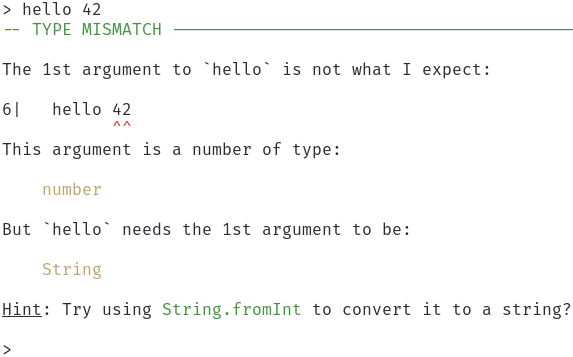
\includegraphics[width=0.7\textwidth]{img/repl_error}
    \caption{Komunikat kompilatora o błędzie}\label{fig:repl_error}
\end{figure}

\subsection{Listy}
Listy są jednymi z najczęściej używanych struktur danych w Elmie.
Ich przeznaczeniem jest trzymanie sekwencji wielu elementów tego samego typu.

Na rysunku~\ref{fig:repl_lists} zostały pokazane przykłady użycia list. Została zdefiniowana lista \texttt{names}, zawierająca trzy elementy typu \texttt{String}, a także tablica \texttt{numbers}, która zawiera 4 liczby (typ \texttt{Int}).

\begin{figure}[H]
    \centering
    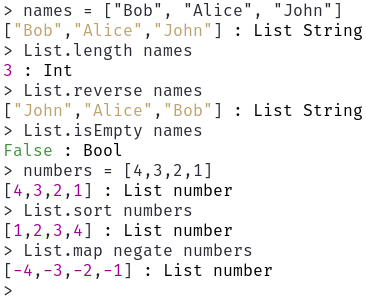
\includegraphics[width=0.5\textwidth]{img/repl_lists}
    \caption{Operacje na listach}\label{fig:repl_lists}
\end{figure}

\subsection{Rekordy}
Rekordy służą do trzymania wielu wartości, gdzie każda z nich jest przypisana do konkretnej nazwy.
Na rysunku~\ref{fig:repl_records} pokazane zostały przykładowe operacje związane z rekordami.
Zdefiniowany został rekord \texttt{bob}, który zawiera informacje o imieniu, nazwisku oraz wieku.

\begin{figure}[H]
    \centering
    \begin{subfigure}{0.7\textwidth}
        \centering
        \caption{Definicja rekordu i dostęp do jednego z pól}\label{fig:repl_record_bob}
        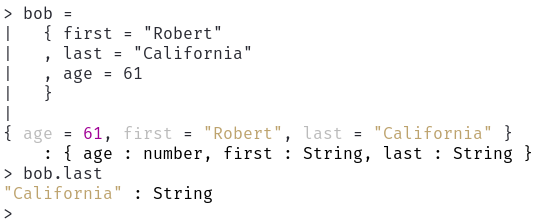
\includegraphics[width=1\textwidth]{img/repl_record_bob}
    \end{subfigure}
    \begin{subfigure}{.7\textwidth}
        \centering
        \caption{Nadpisanie zawartości rekordu}\label{fig:repl_record_update}
        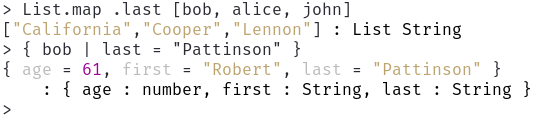
\includegraphics[width=1\textwidth]{img/repl_record_update}
    \end{subfigure}
    \caption{Przykłady pracy z rekordami}\label{fig:repl_records}
\end{figure}

W przypadku rekordów, które zawierają wiele pól, praca z nimi może stawać się problematyczna.
Wygodne może być wtedy wykorzystanie tzw.~,,aliasów typów'', które pozwalają na definicję typu rekordu i korzystanie z niego w skróconej wersji.

Na rysunku~\ref{fig:repl_type_alias} zdefiniowany został nowy typ \texttt{Person}, który jest równoznaczny ze zdefiniowanym na rys.~\ref{fig:repl_record_bob} rekordem \texttt{bob}.
Jednakże tak zdefiniowany typ sprawia, że kod staje się krótszy, bardziej czytelny, a praca z nim dużo wygodniejsza.
\begin{figure}[H]
    \centering
    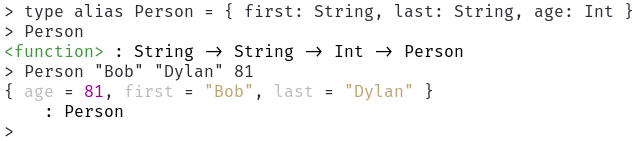
\includegraphics[width=0.85\textwidth]{img/repl_type_alias}
    \caption{Definicja aliasu typu \texttt{Person}}\label{fig:repl_type_alias}
\end{figure}

\section{Aplikacja frontendowa}
W ramach większego projektu zbudowana zostanie strona internetową typu \texttt{startpage}, czyli strona startowa przeglądarki zawierająca najważniejsze i najczęściej używane elementy.
Zaimplementowane zostaną cztery moduły --- Data i czas, pogoda, wyszukiwarka oraz pasek zakładek.

Każda z funkcjonalności będzie dodawana inkrementalnie poprzez dokładanie kolejnych fragmentów kodu do każdej z części architektury Elma, tj. \texttt{Model}, \texttt{Update} oraz \texttt{View}, czyli elementów odpowiedzialnych odpowiednio za stan, logikę i wygląd aplikacji.

Plik źródłowy \texttt{Main.elm} został stworzony w jednym z poprzednich kroków --- należy go otworzyć w swoim wybranym edytorze i przejść do kolejnych kroków.

\subsection{Szkielet aplikacji}
W pierwszej kolejności należy uruchomić aplikację typu~,,Hello World!'', aby upewnić się, że środowisko zostało prawidłowo skonfigurowane.
W załączonym pliku \texttt{Main.elm} znajdują się wszystkie potrzebne do działania klauzule importujące biblioteki podstawowe Elma.
Ponadto zaimplementowana została podstawowa architektura aplikacji.
Aby uruchomić aplikację~,,Hello, World!'' należy otworzyć wiersz poleceń i wykonać polecenie:

\begin{lstlisting}
  $ elm reactor
\end{lstlisting}

Powinien pokazać się następujący widok:

\begin{figure}[H]
    \centering
    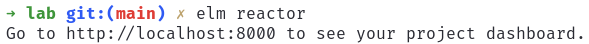
\includegraphics[width=0.9\textwidth]{img/elm_reactor}
\end{figure}

Po otwarciu w przeglądarce adresu \texttt{http://localhost:8000} należy znaleźć plik \texttt{Main.elm} i go otworzyć.
Powinien wyświetlić się napis~,,Hello, World!'' oraz guzik \texttt{Click me!}, który zamienia ciąg tekstowy na~,,Hello, again!''.

Celem dalszych sekcji będzie rozwinięcie tego programu poprzez implementację wymaganych funkcjonalności omówionych na początku instrukcji.

\subsection{Czas}
Do wydobycia informacji o aktualnym czasie wykorzystana zostanie biblioteka \texttt{elm/time}.
W celu zainstalowania tej biblioteki w wierszu poleceń należy wykonać komendę \texttt{\$ elm install elm/time}, a następnie załączyć bibliotekę do tworzonego programu używając klauzuli \texttt{import Time exposing (..)}.

Przechodząc do edycji kodu, pierwszą rzeczą jest zdefiniowanie modelu programu.
Potrzebne będą informacje o strefie czasowej oraz aktualny czas.
W tym celu należy stworzyć nowy typ \texttt{DateTime}, który będzie przechowywał te dane, a następnie dodać go do modelu.

\begin{lstlisting}[language=Elm]
type alias Model =
    { dateTime : DateTime }
type alias DateTime =
    { zone : Time.Zone
    , time : Time.Posix
    }
\end{lstlisting}

Kolejnym krokiem będzie zdefiniowanie typów wiadomości, które może odebrać program.
Do prawidłowego działania zegara potrzebne będzie dostosowanie strefy czasowej oraz pobranie aktualnego czasu.
Oznacza to, że należy zdefiniować dwie wiadomości --- \texttt{AdjustTimeZone} oraz \texttt{Tick}.

\begin{lstlisting}[language=Elm]
type Msg
    = Tick Time.Posix
    | AdjustTimeZone Time.Zone
\end{lstlisting}

Oba typy wiadomości muszą zostać odpowiednio przetworzone w funkcji \texttt{update}.
W obu przypadkach wystarczające będzie nadpisanie stworzonego modelu nowymi wartościami.
Przykład nadpisania rekordu został przedstawiony wcześniej na rys.~\ref{fig:repl_record_update}.

Następnie należy zdefiniować funkcję \texttt{init}, gdzie wskazany zostanie sposób inicjalizacji modelu oraz operacje, jakie mają zostać wykonane na początku programu.
W przypadku daty i czasu należy początkowo wyzerować obie wartości, a następnie pobrać aktualne informacje wykorzystując stworzone przed chwilą wiadomości.

\begin{lstlisting}[language=Elm]
init _ =
    ( Model (DateTime Time.utc (Time.millisToPosix 0))
    , Cmd.batch [ Task.perform AdjustTimeZone Time.here, Task.perform Tick Time.now ]
    )
\end{lstlisting}

Jednakże czas zmienia się z sekundy na sekundę, więc jednorazowe ustawienie wartości modelu niestety nie jest wystarczające --- trzeba aktualizować model co sekundę.
Aby to osiągnąć, wykorzystana zostanie funkcja \texttt{subscriptions}.
Pozwala na nasłuchiwanie zewnętrznych zdarzeń, takich jak kliknięcie myszki, naciśnięcie klawisza na klawiaturze, zmiany w geolokacji lub --- tykanie zegara.

W przypadku tworzonej aplikacji należy co sekundę generować nową wiadomość \texttt{Tick}, która po jej przetworzeniu w funkcji \texttt{update} zaktualizuje aktualny czas w modelu.

\begin{lstlisting}[language=Elm]
subscriptions _ =
    Time.every 1000 Tick
\end{lstlisting}

Ostatnim elementem architektury Elma jest funkcja \texttt{view}, której zadaniem jest wyświetlanie programu na ekranie.

\begin{lstlisting}[language=Elm]
view model =
    { title = "Hello"
    , body =
        [ viewTime model.dateTime
        , viewDate model.dateTime
        ]
    }
\end{lstlisting}

W celu polepszenia czytelności kodu, funkcja \texttt{view} wykorzystuje dwie funkcje pomocnicze --- \texttt{viewTime} oraz \texttt{viewDate}.
Część implementacji jednej z nich została przedstawiona poniżej.
W ramach ćwiczenia należy dokończyć implementację funkcji \texttt{viewDate} oraz stworzyć analogiczną funkcję \texttt{viewTime}.
Ponadto przedstawiony został początek funkcji \texttt{toEnglishWeekday}, która przyjmuje wartość typu \texttt{Time.Weekday} i zwraca typ \texttt{String}, który może zostać następnie wyświetlony w funkcji \texttt{viewDate}.
Implementację tej funkcji także należy dokończyć oraz stworzyć analogiczną funkcję pozwalającą na dekodowanie nazw miesięcy.
Dla lepszego wyglądu zegara warto także stworzyć funkcję dodającą znak 0 dla liczb mniejszych od 10.
\begin{lstlisting}[language=Elm]
viewDate dateTime =
    let
        weekday =
            Time.toWeekday dateTime.zone dateTime.time
        ...
    in
    div [] [ text (toEnglishWeekday weekday) ]
toEnglishWeekday weekday =
    case weekday of
        Mon ->
            "Monday"
        ...
\end{lstlisting}

Jeżeli wszystko udało się pomyślnie, w przeglądarce internetowej powinien wyświetlić się aktualny czas, zmieniający się co sekundę, a pod nim data.
Następnie można przejść do kolejnej sekcji.

\subsection{Pogoda}
Pogoda będzie pobierana wykorzystując zapytania HTTP do API portalu OpenWeatherMap\@.
Potrzebne będą do tego dwie biblioteki --- \texttt{elm/http} do wysłania zapytania oraz \texttt{elm/json} do odebrania i przetworzenia odpowiedzi w formacie JSON\@.
Podobnie jak poprzednio, należy je zainstalować używając poleceń:
\begin{lstlisting}
  $ elm install elm/http
  $ elm install elm/json
\end{lstlisting}
Następnie należy dodać do pliku \texttt{Main.elm} następujące klauzule:

\begin{lstlisting}[language=Elm]
import Http
import Json.Decode exposing (..)
\end{lstlisting}

Przed przejściem do edycji kodu programu należy założyć darmowe konto na stronie \href{https://openweathermap.org/}{OpenWeatherMap}, a następnie wygenerować klucz API, który będzie konieczny do prawidłowego działania aplikacji.
Po stworzeniu prywatnego klucza API można przejść do kolejnych kroków.

W przypadku pogody potrzebne będzie stworzenie dwóch nowych typów: jeden będzie zawierał informacje o faktycznym stanie pogody, tj.~temperatura i krótki opis słowny, a drugi informacje o statusie zapytania HTTP\@.

\begin{lstlisting}[language=Elm]
type WeatherStatus
    = Failure String
    | Loading
    | Success Weather
type alias Weather =
    { description : String
    , temperature : Float
    }
\end{lstlisting}

Powyższy typ \texttt{WeatherStatus} należy dodać do głównego modelu.
Ponadto należy zdefiniować w programie dane potrzebne do wysłania zapytania, a następnie wykorzystać je w funkcji odpowiedzialnej za wysłanie zapytania GET do OpenWeatherAPI\@.
Są to:
\begin{itemize}[noitemsep,topsep=0pt]
    \item URL do wysłania zapytania
    \item Prywatny klucz API do OpenWeatherMap
    \item Miasto
    \item Jednostki
\end{itemize}
Przykład implementacji został przedstawiony poniżej:

\begin{lstlisting}[language=Elm]
getWeather =
  Http.get
    { url = weatherApi ++ ("&q=" ++ city) ++ ("&units=" ++ unit) ++ ("&appid=" ++ apiKey)
    , expect = Http.expectJson GotWeather weatherDecoder
    }
\end{lstlisting}
Szczegóły użycia API opisane są w \href{https://openweathermap.org/current#name}{dokumentacji OpenWeatherMap}.

Z perspektywy Elma najważniejsze jest sprecyzowanie rodzaju zapytania (tutaj GET) oraz adresu URL, na który ma został wysłane zapytanie.
Konieczne jest także określenie formy spodziewanej odpowiedzi (JSON), a także przekazanie funkcji jej dekodującej.
Na końcu należy przekazać rodzaj wiadomości do wygenerowania po odebraniu odpowiedzi (\texttt{GotWeather}).

A jak wygląda funkcja i dekodująca i do czego służy?
Przykład prostego dekodera został przedstawiony poniżej.
Celem dekodera jest przetworzenie pliku w formacie JSON w taki sposób, aby był zrozumiały dla Elma.
Należy w nim określić nazwy oczekiwanych pól oraz opisać jak się do nich dostać.

Funkcja \texttt{personDecoder} spodziewa się trzech wartości --- dwóch ciągów znaków i jednej liczby, które znajdują się w polach nazwanych odpowiednio \texttt{first}, \texttt{last} oraz \texttt{age}.
Typ \texttt{Person} został stworzony na rys.~\ref{fig:repl_record_update} i zawiera w sobie takie same typy jak dekoder.
Oznacza to, że taka odpowiedź JSON powinna zostać prawidłowo zmapowana na typ \texttt{Person}.
\begin{lstlisting}[language=Elm]
personDecoder =
  map3 Person
      (field "first" string)
      (field "last" string)
      (field "age" int)
\end{lstlisting}

W ramach ćwiczenia należy zaimplementować funkcję \texttt{weatherDecoder}, która zmapuje odpowiednie pola z odpowiedzi JSON na typ \texttt{Weather} zaimplementowany wcześniej w modelu.

W przypadku wiadomości \texttt{Msg} sytuacja będzie podobna jak przy tworzeniu typów --- potrzebny będzie jeden rodzaj wiadomości odpowiedzialny za wysłanie zapytania oraz drugi odpowiedzialny za jego odebranie i odpowiednie zaktualizowanie modelu na podstawie danych odebranych z dekodera.

\begin{lstlisting}[language=Elm]
type Msg
    = ...
    | UpdateWeather
    | GotWeather (Result Http.Error Weather)
\end{lstlisting}

\begin{lstlisting}[language=Elm]
update msg model =
  case msg of
    ...
    UpdateWeather ->
      ( { model | weatherStatus = Loading }, getWeather )
    GotWeather result ->
      case result of
        Ok weather ->
          ( { model | weatherStatus = Success weather }, Cmd.none )
        Err _ ->
          ( { model | weatherStatus = Failure "Error: Couldn't retrieve weather data" }, Cmd.none)
\end{lstlisting}


\subsection{Wyszukiwarka}
Wyszukiwarka jest jedną z prostszych funkcjonalności do implementacji.
Potrzebne będzie jedynie stworzenie pola tekstowego, gdzie użytkownik może wpisać wybraną frazę, oraz jego odpowiednie obsłużenie.
Po wpisaniu frazy i wciśnięciu klawisza Enter użytkownik powinien zostać przeniesiony do strony wyszukiwarki z wyszukanym wpisanym już wcześniej hasłem.

Można zauważyć, że tym razem do modelu należy dołożyć jedynie jedną wartość --- ciąg znaków wpisany przez użytkownika.
Wiadomości typu \texttt{Msg} natomiast będą dwie --- jedna standardowo odpowiedzialna za zaktualizowanie modelu, a druga za przekierowanie strony do wyszukiwarki.
Przekierowanie odbywa się za pomocą funkcji \texttt{load} z biblioteki \texttt{Navigation}, która powinna już być załączona do programu w początkowym szkielecie.
Poniżej zostały przedstawione propozycje implementacji wiadomości \texttt{Search} obsługującej przekierowanie do wyszukiwarki oraz funkcji \texttt{viewSearchBar} wyświetlającej pole tekstowe.
Dodatkowo zaimplementowana została funkcja \texttt{onEnter} pozwalająca na wykrycie czy użytkownik wcisnął klawisz Enter.
\begin{lstlisting}[language=Elm]
Search ->
  ( model
  , Nav.load ("https://google.com/search?q=" ++ model.searchText)
  )
\end{lstlisting}
\begin{minipage}{.56\textwidth}
\begin{lstlisting}[language=Elm]
onEnter msg =
  let
    isEnter code =
      if code == 13 then
        succeed msg
      else
        fail "not ENTER"
  in
  on "keydown" (andThen isEnter keyCode)
\end{lstlisting}
\end{minipage}\hfill
\begin{minipage}{.38\textwidth}
\begin{lstlisting}[language=Elm]
viewSearchBar =
  div []
    [ input
      [ type_ "text"
      , placeholder "Search"
      , onInput UpdateField
      , onEnter Search
      ] []
    ]
\end{lstlisting}
\end{minipage}\hfill

W ramach ćwiczenia należy zaimplementować model oraz rozszerzyć funkcję \texttt{update} o dwie nowe wiadomości, jak i główną funkcję \texttt{view} o przedstawioną wyżej propozycję \texttt{viewSearchBar}.
Po prawidłowym złączeniu wszystkich fragmentów kodu program powinien się kompilować i wyświetlać nowy pasek pola tekstowego, a po wciśnięciu klawisza Enter strona powinna zostać przekierowana do wyszukiwarki Google.

Jeżeli wszystko udało się zaimplementować pomyślnie, można przejść do kolejnego kroku.

\subsection{Zakładki}
W dalszej części implementacji
Do prawidłowego działania zakładek potrzebne będzie stworzenie dwóch dodatkowych plików --- \texttt{bookmarks.js} oraz \texttt{index.html}.
Pierwszy posłuży do trzymania listy zakładek, gdzie każda składa się z adresu URL oraz nazwy, która zostanie wyświetlona na tworzonej stronie.
Natomiast drugi plik \texttt{index.html} potrzebny będzie do załadowania do programu poprzedniego pliku z zakładkami jak i pliku wynikowego stworzonego przez kompilator Elma z użyciem następującej komendy:
\begin{lstlisting}
  $ elm make src/MainBookmarks.elm --output=assets/elm.js
\end{lstlisting}

W sekcji \texttt{<head>} pliku \texttt{index.html} należy załączyć plik z zakładkami oraz wynikowy plik kompilatora.
W sekcji \texttt{<body>} należy dodać fragment kodu przedstawiony poniżej, który pozwoli na wykorzystanie programu w Elmie razem z zewnętrznym plikiem HTML\@.

\noindent
\begin{minipage}{.41\textwidth}
\begin{lstlisting}[language=html]
<head>
  <script
    src="assets/elm.js">
  </script>
  <script
    src="assets/bookmarks.js">
  </script>
</head>
\end{lstlisting}
\end{minipage}\hfill
\begin{minipage}{.55\textwidth}
\begin{lstlisting}[language=html]
<body>
  <div id="app"></div>
  <script>
    var app = Elm.Main.init({
      node: document.getElementById("app"),
      flags: bookmarks,
    });
  </script>
</body>
\end{lstlisting}
\end{minipage}\hfill

Po otwarciu pliku \texttt{index.html} z użyciem programu \texttt{elm reactor} aplikacja wraz z zakładkami powinna pojawić się na ekranie.

\subsection{Style}
W załączonym pliku \texttt{styles.css} znajdują się kaskadowe arkusze stylów, które mogą zostać wykorzystane wraz ze stworzoną aplikacją.
W tym celu należy odpowiednio zmienić w programie funkcje odpowiedzialne za wyświetlanie elementów, dodając do nich tagi \texttt{div[][]}.
Funkcja \texttt{div} przyjmuje dwa argumenty: listę atrybutów oraz listę elementów HTML\@.
W tej części należy skupić się na pierwszym argumencie, gdyż dotychczas nie był on jeszcze używany.
Atrybuty HTML to np. \texttt{class}, \texttt{id} oraz \texttt{style}.

Na przykładzie głównej funkcji \texttt{view}, wykorzystanie klasy \texttt{container} wygląda następująco:
\begin{lstlisting}[language=Elm]
view model =
  { ...
  , body =
    [ div [ class "container" ]
      [ viewTime model.clockTime
        ... ] ]
  }
\end{lstlisting}

Jako, że plik \texttt{styles.css} został dostarczony w załączniku, w ramach ćwiczenia w aplikacji wystarczy jedynie dodać w odpowiednich miejscach funkcje \texttt{div} wraz z pasującymi atrybutami, które zostały zdefiniowane w arkuszu stylów.

\subsection{Efekt}
Jeżeli wszystkie funkcjonalności zostały prawidłowo zaimplementowane, a arkusze stylów właściwie użyte w programie, finalna aplikacja powinna wyglądać następująco:
\begin{figure}[H]
    \centering
    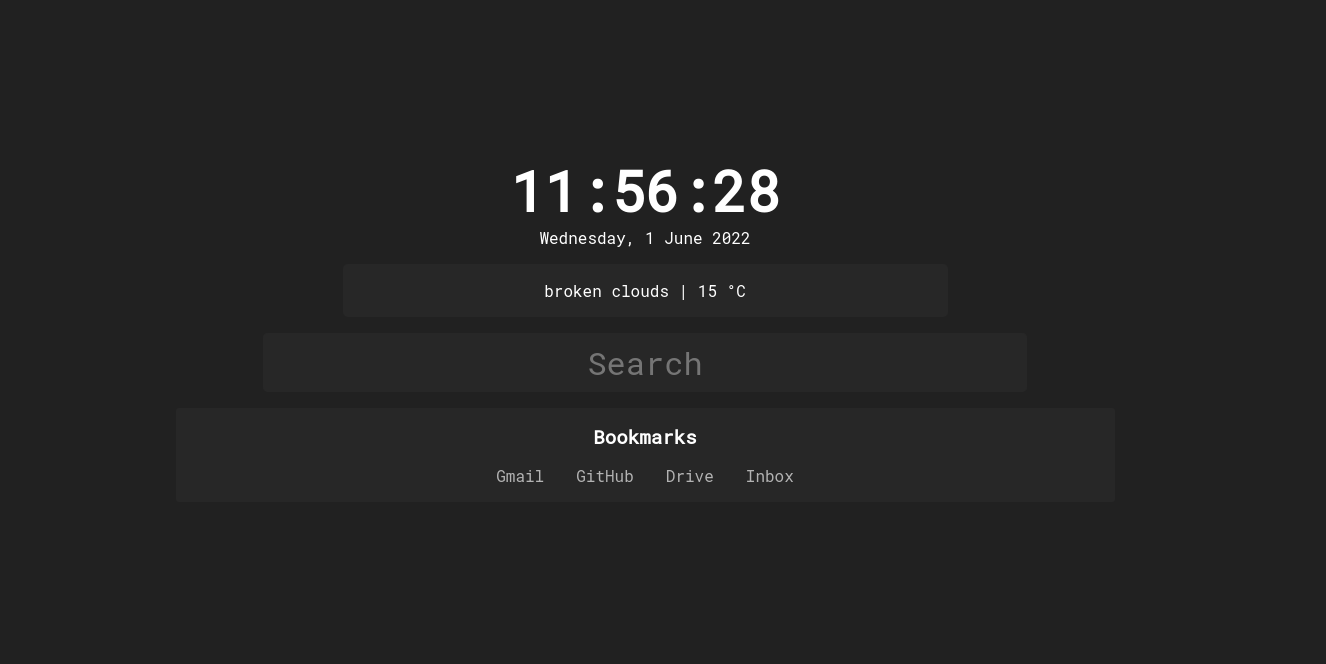
\includegraphics[width=0.9\textwidth]{img/final_app.png}
\end{figure}

% ---------------------------------------------------------------------------------------------------------------------

\end{document}

